\section{Optimizing Hyperparameter Search} \label{sec-hyperparam-optimization}
In some workloads, instead of training a model on the data, the user performs a hyperparameter search operation.
In the hyperparameter search, the user defines a space of possible hyperparameters for the model and train multiple models (sometimes hundreds or thousands) to find the model with the hyperparameters that provides the best performance.
The three common search strategies are grid search, random search, and sequential model-based optimization (guided search).
In this section, we propose several optimizations for hyperparameter search operations.
\subsection{Grid Search}
In the grid search approach, the user first defines a grid of hyperparameter values (1 dimension for every hyperparameter of the model).
The search process then proceeds to use the values at each point of the grid, trains a model to the completion, and stores the quality metrics of the model.
After executing the training operation for every point in the grid, the model with the best quality metric is chosen as the final model.

To optimize the grid search operation, we first transform the grid into several model training operation through a simple process called grid unpacking.
After unpacking, the reuse optimizations techniques discussed in Section \ref{sub-sub-model-reuse} can be applied.

\subsubsection{Grid unpacking}
To apply the reuse operations in the grid search, we must first unpack the grid.
When presented with a grid search operation (either in the workload or the experiment database), we first extract every point in the grid as one run of the model training operation.
Then, we add each run as a separate operation to the experiment graph.
Figure \ref{fig-grid-unpacking} shows an example of grid unpacking for a simple SVM Model which has the two hyperparameters penalty (C) and learning rate.

\begin{figure}
\centering
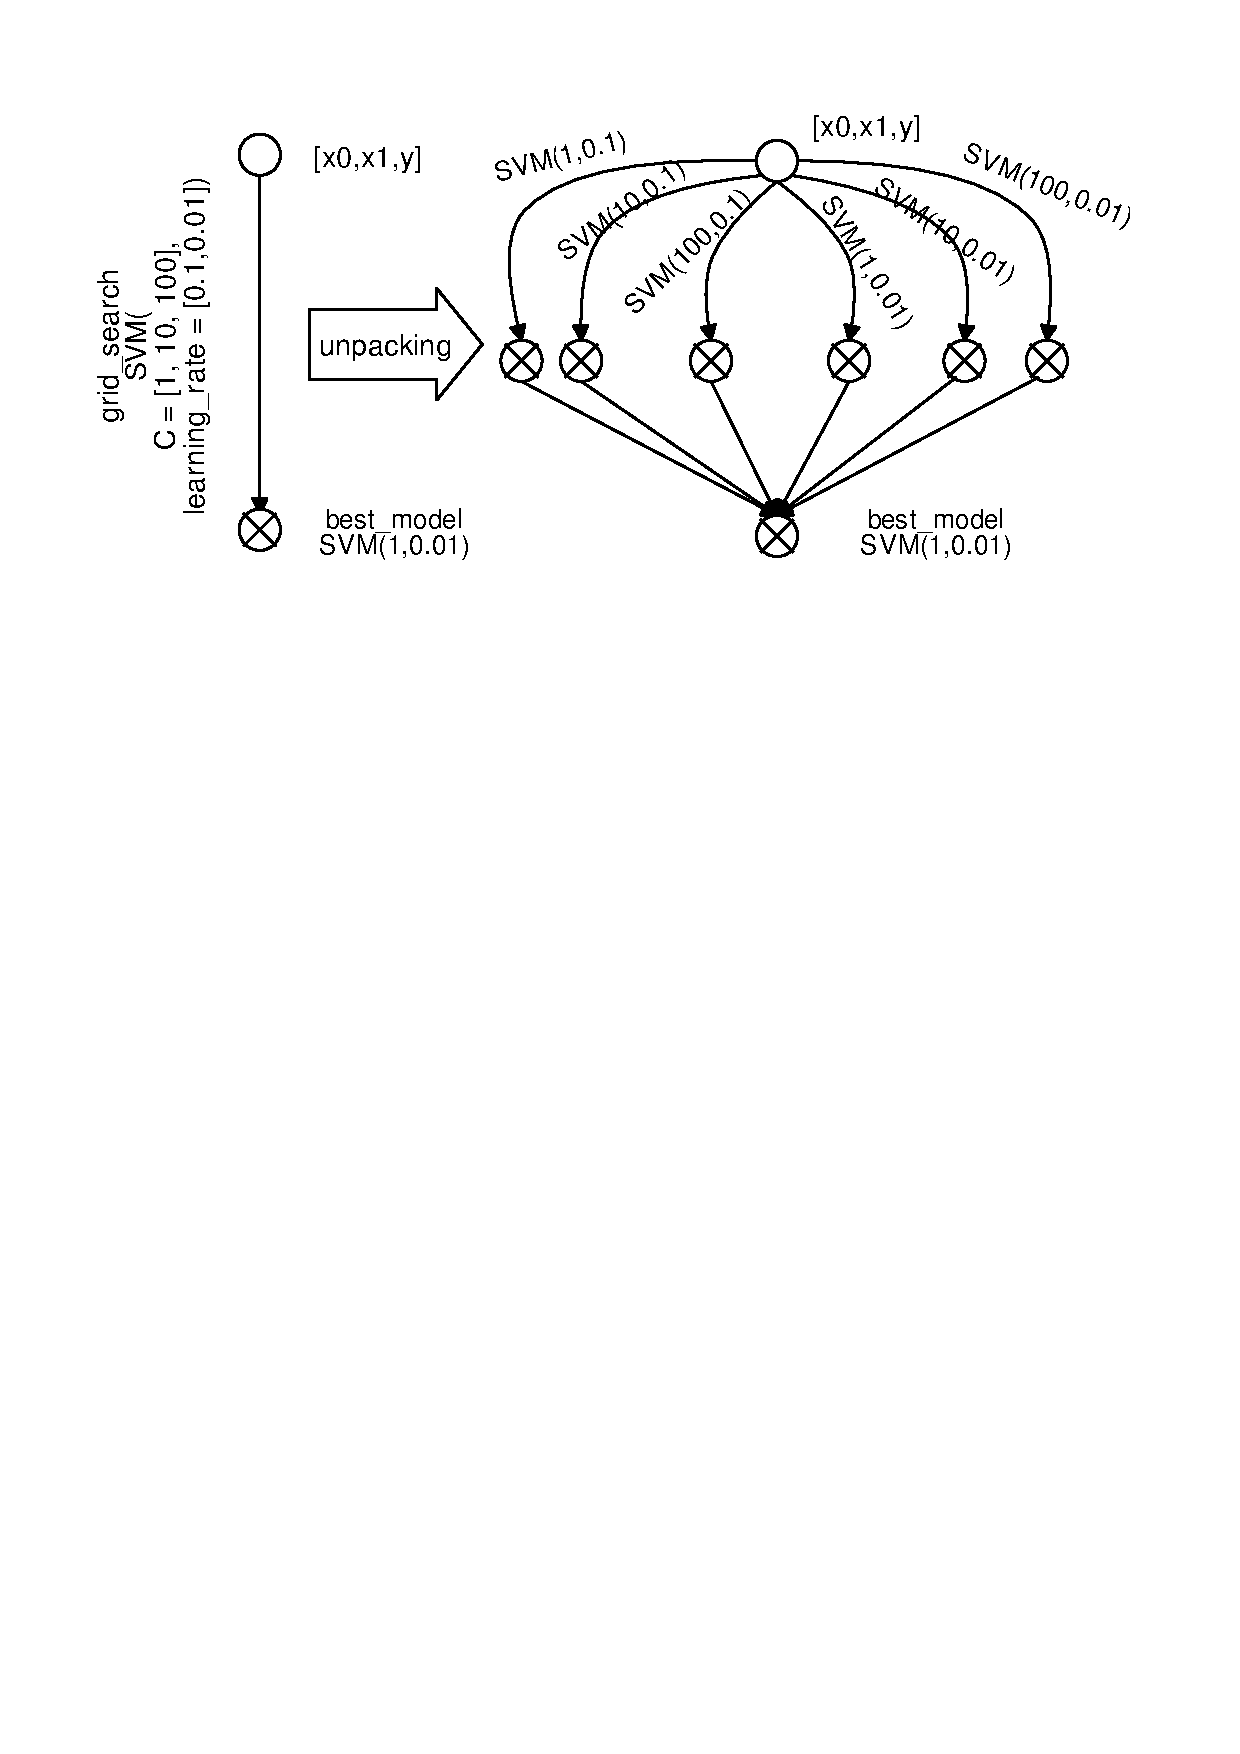
\includegraphics[width=\columnwidth]{../images/grid-unpacking}
\caption{Result of unpacking on a small grid for SVM model. The hyperparameters are C=[1, 10, 100] and learning rate=[0.1, 0.01]}
\label{fig-grid-unpacking}
\end{figure}


\subsection{Random Search}

\subsection{Sequential Model-based Optimization}

\subsubsection{Automatic Search Space Definition}\label{sub-section-automatic-search-definition}
Extracting the parameter ranges from the experiment database can give us an estimate for defining the search space over undefined hyperparameters, thus, making the search process easier for users that do not have in-depth knowledge of machine learning.

\subsubsection{Warm Starting the Optimization}
Here, we discuss how we use the experiment database to warm start the search process., thus, reducing the search time and increasing the probability of finding very good hyperparameter settings.

\subsubsection{Avoiding Local Optima}
Warm starting for advanced hyperparameter optimization have the benefit of reducing the overhead of computing many trials.
However, inserting the data from the experiment database into the optimization process may lead the search into local optima.
Hence, the search process may focus on exploiting specific areas and avoid exploring the space.
This could decrease the chance of finding the best hyperparameter setting.


\subsubsection{Adaptive warmstarting}
Many sets of hyperparameters are similar and may force the search to local minima.
By adaptively selecting points, we can still increase the efficiency of search without forcing the search into local regions.

\subsubsection{Explorer unit}
The explorer is a bot that explorers beyond the defined search space.
Using pipelines defined by experts, the explorer can help in the exploration of the search space.
Ultimately, by automatically exploring the space, not only we can help in avoiding the local optima but possibly we can also help redefine the search space as described in Section \ref{sub-section-automatic-search-definition}.


